\documentclass[11pt]{article}
\usepackage{amsmath, amssymb, amsthm}
\usepackage[retainorgcmds]{IEEEtrantools}

\usepackage[pdftex]{graphicx}
\usepackage{tikz}
\usetikzlibrary{intersections}

\usepackage{marginnote}
\usepackage{endnotes}

\usepackage{fancyhdr}

%Listings stuff
\usepackage{listings}
\usepackage{lstautogobble}
\usepackage{color}

\definecolor{gray}{rgb}{0.5,0.5,0.5}
\lstset{
basicstyle={\small\ttfamily},
tabsize=3,
numbers=left,
numbersep=5pt,
numberstyle=\tiny\color{gray},
stepnumber=2,
breaklines=true
}

%Properly formatted differential 'd'
\newcommand{\ud}{\, \mathrm{d}}

%Format stuff
\pagestyle{fancy}
\headheight 35pt

%Header info
\chead{\Large \textbf{Propositional Logic}}
\lhead{}
\rhead{}

\begin{document}
\section{Introduction}
	\textbf{Axioms} are statements accepted without proof. The axiomatic method can be used to determine other truths by applying logic to a set of existing axioms.
	
	\textbf{Logic} is a formal system for expressing truth and falsity and provides a systematic, tractable method of reasoning from given axioms to \textbf{propositions} or \textbf{theorems}.
	
	\subsection{Propositional Statements}
		A \textbf{statement} is a declaration that is either true or false.
		\begin{equation}
			s := statement::s\rightarrow\{0, 1\}
		\end{equation}
		There are three fundamental operators for statements.
		\begin{IEEEeqnarray}{rCl}
			\text{(or) }& \vee & :s\times s\rightarrow\{false,true\}\\
			\text{(and) }&\wedge & :s\times s\rightarrow\{false,true\}\\
			\text{(not) }&\lnot &:s\rightarrow\{false, true\}
		\end{IEEEeqnarray}
		
		The truth or falsity of any statement depends upon its \textbf{context}, which can be visualized as the values that are associated with each variable in a statement. For example, the context of $a\vee b$ is either $a=true$ or $b=true$, but the context of $a\wedge b$ is $a=true$ and $b=true$.
		
	\subsection{Logical Equivalence}
		Can prove logical equivalence with truth tables or by induction. When using a truth table, the number of \textit{necessary rows} is determined by the number of variables. Read terminal row values as \textit{products} and columns as \textit{co-products}.
		
		Given any statements $p,q,\text{ and } r$, a tautology $t$, and a contradiction $c$, some logical equivalences are summarized below. Statements and operators are also commutative, associative, and distributive.
		\begin{center}
		\begin{tabular}{l|cc}
			Law			&	Case 1			&	Case 2\\\hline
			De Morgan's	& $\lnot(p\wedge q)\equiv \lnot p\vee \lnot q$ & $\lnot(p\vee q)\equiv\lnot p\wedge\lnot q$\\
			Absorption	& $p\vee(p\wedge q)\equiv p$	& $p\wedge(p\vee q)\equiv p$\\
			Distributive	&	$p\wedge(q\vee r)\equiv(p\wedge q)\vee(p\wedge r)$	&	$p\vee(q\wedge r)\equiv(p\vee q)\wedge(p\vee r)$
		\end{tabular}
		\end{center}
		
	\subsection{Boolean Algebra}
		When doing algebra with logical statements, consider all conjunctions ($\vee$) as addition signs and all disjunctions ($\wedge$) as multiplication signs.
		\begin{IEEEeqnarray}{Ll}
			& (p\wedge q)\vee(p\wedge r)\\
			= & (p\times q)+(p\times r)\\
			= & p\times(q + r)\\
			= & p\wedge(q\vee r)
		\end{IEEEeqnarray}
		
\section{Logical Implication}
	\textbf{Logical implication} is a \textit{directional} operator that points from an antecedant, or hypothesis, to a necessary condition, or conclusion. Implication captures the notion of an action depending on the success or failure of another action (If it rains, then I bring an umbrella).
	\begin{equation}
		p\Rightarrow q
	\end{equation}
	\begin{center}
	\begin{tabular}{cc|c}
		p & q & $p\Rightarrow q$\\\hline
		&&\\
		T & T & T\\
		F & T & T\\
		T & F & F\\
		F & F & T
	\end{tabular}
	\end{center}
	
	The last case is called a \textbf{vacuous truth} because we assume the implication to be true unless proved otherwise. An implication is false just in the case that its hypothesis is true, but its conclusion is false, i.e. the necessary condition is not satisfied. Analyzing the truth table gives the following.
	\begin{equation}
		p\Rightarrow q \equiv \lnot p\vee q
	\end{equation}
	
	Importantly, no relationship need exist between the antecedent and necessary condition (``If the moon is made of cheese, then $\emptyset$ is the subset of all sets'').
	
	\subsection{Transitivity}
		\begin{equation}
			p\Rightarrow q, q\Rightarrow r\vdash p\Rightarrow r
		\end{equation}
		
		By derivation:
		\begin{IEEEeqnarray*}{rCl}
			(p\Rightarrow q)\wedge(q\Rightarrow r) & \stackrel{?}{\vdash} & p\Rightarrow r\\
			(\lnot p\vee q)\wedge(\lnot q\vee r) & = &\\
			\lnot p\vee(q\wedge\lnot q)\vee r & = &\\
			(\lnot\vee c)\vee r & = &\\
			(\lnot p)\vee r & = &\\
			p\Rightarrow r & \equiv & p\Rightarrow r
		\end{IEEEeqnarray*}
		
	\subsection{Negation}
		\begin{equation}
			\lnot(p\Rightarrow q)\equiv p\wedge\lnot q
		\end{equation}
		
	\subsection{Contrapositive}
		If the positive is true, the contrapositive is also true.
		\begin{equation}
			\lnot q\Rightarrow\lnot p
		\end{equation}
		
	\subsection{Biconditional}
		In English, equivalent to "p, if and only if q." Only true when p and q are both true or both false.
		\begin{IEEEeqnarray}{rCl}
			p\leftrightarrow q & \equiv & [(q\Rightarrow q)\wedge(q\Rightarrow p)]\\
			\nonumber p\leftrightarrow q &\equiv &(\lnot p\vee q) \wedge (\lnot q\vee p)\\
			\nonumber & \equiv &(\lnot p\wedge\lnot q)\vee(p\wedge q)
		\end{IEEEeqnarray}
		
\section{Logical Circuits}
	Logical statements can be represented by circuitry with switches to indicate the state of variables - on is true, off is false, or vice versa if the variables is negated. Then, a logical conjunction (and) is two switches wired in series, and a logical disjunction (or) is two switches wired in parallel.
	
	It is also possible to represent the all logic using three basic \textbf{logic gates}: AND, OR, and NOT (Figure \ref{fig:logicgate}).
	
	\begin{figure}[htb]
		\centering
		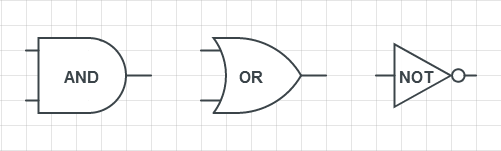
\includegraphics[width=0.8\textwidth]{logicgates.png}
		\caption{Logic gates}
		\label{fig:logicgate}
	\end{figure}	
	
	\subsection{Simplifying Expressions}
		Given a complex truth, it is possible to construct a logical expression and circuit to match.. There are two ways to simplify: with conjunctions and with a Karnaugh map.
		\begin{center}
		\begin{tabular}{cccc|c}\label{truthtab}
			A&B&C&D&$f(A,B,C,D)$\\\hline
			0&0&0&0&0\\
			0&0&0&1&0\\
			0&0&1&0&0\\
			0&0&1&1&0\\
			0&1&0&0&0\\
			0&1&0&1&0\\
			0&1&1&0&1\\
			0&1&1&1&0\\
			1&0&0&0&1\\
			1&0&0&1&1\\
			1&0&1&0&1\\
			1&0&1&1&1\\
			1&1&0&0&1\\
			1&1&0&1&1\\
			1&1&1&0&1\\
			1&1&1&1&0
		\end{tabular}
		\end{center}
	
		To construct the corresponding logical expression with conjunctions, isolate all of the rows where $f(A,B,C,D) = 1$ and join them together. This method is called the \textbf{sum-of-products} method. 
		\subsubsection{Karnaugh Maps}
			Example based on truth table above.
			
			\begin{figure}[htb]
				\centering
				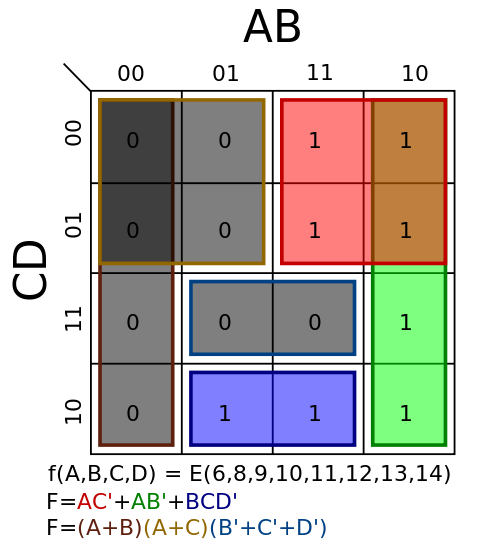
\includegraphics[width=0.7\textwidth]{kmap.png}
				\caption{K-map for Table \ref{truthtab}}
				\label{fig:kmap1}
			\end{figure}
			
			The first step is to isolate rectangles containing 1's. In this example, there are three such rectangles, highlighted in red, green and blue (brown is the intersection between the red and green boxes).
			
			The red grouping is $A\wedge\lnot C$:
			\begin{itemize}
				\item The variable A is the same and is equal to 1 throughout the box, therefore it should be included in the algebraic representation of the red minterm.
				\item Variable B does not maintain the same state (it shifts from 1 to 0), and should therefore be excluded.
				\item C does not change. It is always 0 so NOT-C should be included.
				\item D changes, so it is excluded as well.
			\end{itemize}

			For the green grouping, A and B maintain the same state, while C and D change. B is 0 and has to be negated before it can be included. Thus the second term is $A\wedge\lnot B$. In the same way, the blue grouping gives the term $B\wedge C\wedge\lnot D$. The solutions of each grouping are combined thus 
			\begin{equation}
				(A\wedge\lnot C)\vee(A\wedge\lnot B)\vee(B\wedge C\wedge\lnot D)
			\end{equation}
			
	\subsection{Adders}
		\subsubsection{Half-Adder}
			The half-adder is the most basic adder, and does not combine the final carry bit (if it exists) with the sum.
			\begin{IEEEeqnarray}{rCl}
				sum & = & (P\vee Q)\wedge \sim(P\wedge Q)\\
				carry & = & (P\wedge Q)
			\end{IEEEeqnarray}
			
			\begin{figure}[htb]
				\centering
				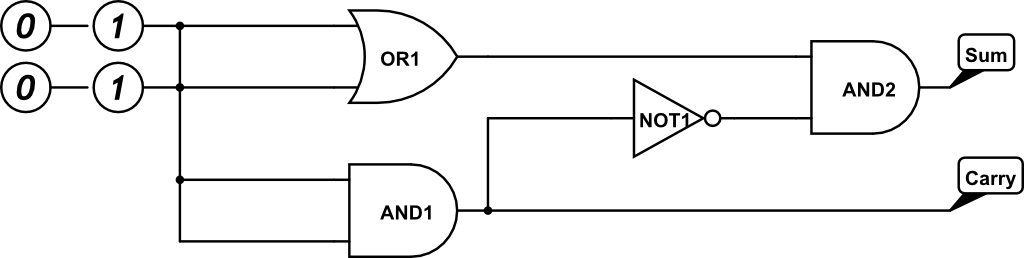
\includegraphics[width=0.8\textwidth]{half-adder.png}
				\caption{The half-adder.}
				\label{fig:half-adder}
			\end{figure}
			
		\subsubsection{Full Adder}
			\begin{figure}[htb]
				\centering
				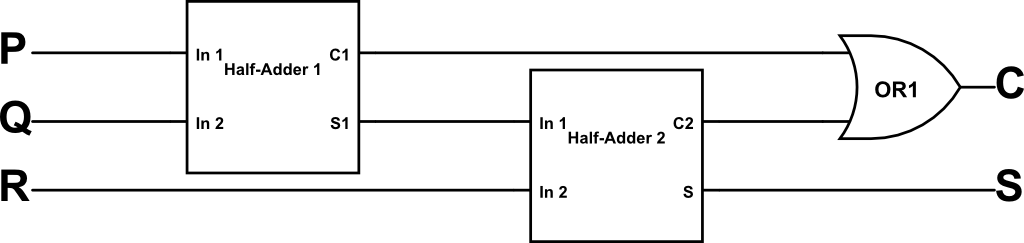
\includegraphics[width=0.8\textwidth]{full-adder.png}
				\caption{The full-adder.}
				\label{fig:full-adder}
			\end{figure}
			
\section{Binary Number Systems}
	\subsection{Twos-complement}
		The \textbf{one's complement} of a binary number is constructed by flipping all of its bits. The one's complement of any positive $n$ acts like its negative in most arithmetic. However, with one's complement, we run into troubles like negative zero.
		
		In \textbf{two's complement}, we invert a binary number by forming the one's complement, then adding 1. The two's complement is also an \textbf{involution}, meaning a function that is its own inverse.
		\begin{equation}
			-a = [(2^n - 1) - a] + 1
		\end{equation}
		In bitwise terms, assuming all numbers are padded with 0 on the left.
		\begin{equation}
			-a =\ \sim a + 1
		\end{equation}
		When adding a positive and negative number in two's complement, the carry bit denotes the sign of the result - 0 for negative, 1 for positive.
	
%	\begin{center}
%	\begin{tikzpicture}
%		[scale=3,line cap=round,
%		%Styles
%		axes/.style=,
%		important line/.style={very thick},
%		information text/.style={rounded corners,fill=red!10,inner sep=1ex},
%		dot/.style={circle,inner sep=1pt,fill,label={#1},name=#1}			
%		]
%		
%		%Colors
%		\colorlet{anglecolor}{green!50!black}	%angle arcs/lines
%		
%		%The graphic
%	\end{tikzpicture}
%	\end{center}

%	\begin{figure}[htb]
%		\centering
%		\includegraphics[width=0.8\textwidth]{filename.eps}
%		\caption{Caption.}
%		\label{fig:figure}
%	\end{figure}

%		\def\enotesize{\normalsize}
%		\theendnotes
\end{document}